\documentclass[11pt,a4paper]{ctexart}

\usepackage{amsmath,amssymb,bm}
\usepackage{geometry}
\usepackage{enumitem}
\usepackage{fancyhdr}
\usepackage{lastpage}
\usepackage{xcolor}
\usepackage{tcolorbox}
\usepackage{tikz}
\usepackage{titlesec}
\usepackage{microtype}
\usepackage{graphicx}
\usetikzlibrary{arrows.meta,calc}

\geometry{left=2.15cm,right=2.15cm,top=2.0cm,bottom=2.0cm}
\setlength{\parindent}{2em}
\setlength{\parskip}{0.25em}
\linespread{1.12}
\graphicspath{{figures/}}

\definecolor{mainblue}{RGB}{39,91,150}
\definecolor{lightblue}{RGB}{232,241,252}
\definecolor{darkgray}{RGB}{65,65,65}
\definecolor{lightgray}{RGB}{245,246,248}

\titleformat{\section}{\large\bfseries\color{mainblue}}{}{0em}{}[\titlerule]
\titleformat{\subsection}{\normalsize\bfseries\color{darkgray}}{}{0em}{}
\titlespacing*{\section}{0pt}{0.9em}{0.45em}
\titlespacing*{\subsection}{0pt}{0.65em}{0.25em}

\setlist[enumerate]{leftmargin=2.2em,itemsep=0.25em,topsep=0.25em}
\setlist[itemize]{leftmargin=2.0em,itemsep=0.2em,topsep=0.2em}

\pagestyle{fancy}
\fancyhf{}
\lhead{\small 格物助航｜每日一练}
\rhead{\small 2026.6.19}
\cfoot{\small 第 \thepage\ 页 / 共 \pageref{LastPage} 页}
\renewcommand{\headrulewidth}{0.4pt}

\newtcolorbox{problemBox}{
  colback=lightblue,
  colframe=mainblue,
  arc=2mm,
  boxrule=0.7pt,
  left=1.0em,
  right=1.0em,
  top=0.8em,
  bottom=0.8em,
  before skip=0.6em,
  after skip=0.8em
}

\newtcolorbox{tipBox}{
  colback=lightgray,
  colframe=darkgray,
  arc=1.5mm,
  boxrule=0.5pt,
  left=0.9em,
  right=0.9em,
  top=0.6em,
  bottom=0.6em,
  before skip=0.5em,
  after skip=0.5em
}

\newcommand{\dd}{\mathrm{d}}

\begin{document}

\begin{center}
  {\Large\bfseries\color{mainblue} 格物助航｜每日一练}\par
  \vspace{0.25em}
  {\large 电磁学第八章：麦克斯韦电磁场理论}\par
  \vspace{0.35em}
  {\small 2026年6月19日}\par
  \vspace{0.35em}
  {\small 编写：罗琦皓}
\end{center}

\vspace{-0.3em}

\begin{problemBox}
\noindent\textbf{题目}\quad
真空中两块半径为 $R$ 的圆形平行板构成电容器，忽略边缘效应。放电过程中，两板间电场在空间上近似均匀，方向沿 $+x$，大小随时间按
\[
  E(t)=E_0e^{-t/\tau}
\]
变化。求：
\begin{enumerate}
  \item 两板间的位移电流密度 $\bm J_d$，以及穿过整个极板面积的位移电流 $I_d$；
  \item 距中心轴线为 $r$ 处的磁感应强度大小 $B(r,t)$，分别讨论 $0<r<R$ 与 $r>R$；
  \item 磁场方向应如何判断；
  \item 这道题体现了麦克斯韦修正安培环路定理的哪一点。
\end{enumerate}
\end{problemBox}

\begin{center}
  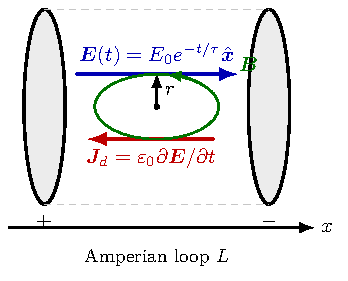
\includegraphics[width=0.58\textwidth]{displacement_current.pdf}\par
  {\small 电场减小时，位移电流密度方向与 $\bm E$ 方向相反，磁场线绕中心轴成同心圆。}
\end{center}

\section*{详细解法}

\subsection*{一、位移电流密度与总位移电流}

真空中
\[
  \bm D=\varepsilon_0\bm E.
\]
位移电流密度定义为
\[
  \bm J_d=\frac{\partial \bm D}{\partial t}
  =\varepsilon_0\frac{\partial \bm E}{\partial t}.
\]
题中
\[
  \bm E(t)=E_0e^{-t/\tau}\hat{\bm x},
\]
所以
\[
  \boxed{
  \bm J_d
  =-\frac{\varepsilon_0E_0}{\tau}e^{-t/\tau}\hat{\bm x}.}
\]
负号说明位移电流密度方向沿 $-x$。

若取面积矢量方向为 $+x$，则穿过整个极板面积的位移电流为
\[
  I_d=\iint \bm J_d\cdot \dd\bm S
  =-\frac{\varepsilon_0E_0}{\tau}e^{-t/\tau}\pi R^2 .
\]
因此位移电流大小为
\[
  \boxed{|I_d|
  =\varepsilon_0\pi R^2\frac{E_0}{\tau}e^{-t/\tau}.}
\]

\subsection*{二、用修正安培环路定理求 $B(r,t)$}

麦克斯韦修正后的安培环路定理为
\[
  \oint_L \bm B\cdot \dd\bm l
  =\mu_0\left(I_{\text{传}}+\frac{\dd\Phi_D}{\dd t}\right).
\]
两极板间没有传导电流穿过所取圆面，所以 $I_{\text{传}}=0$。由于电场具有轴对称性，磁感应线是绕中心轴的同心圆。取半径为 $r$ 的圆形安培环路，则圆周上 $B$ 大小相等，方向沿切向。

\subsection*{三、$0<r<R$ 的情况}

环路所围面积为 $\pi r^2$，电位移通量为
\[
  \Phi_D=\varepsilon_0E(t)\pi r^2.
\]
代入安培环路定理：
\[
  B\cdot 2\pi r
  =\mu_0\varepsilon_0\pi r^2\frac{\dd E}{\dd t}.
\]
如果只求大小，则
\[
  \boxed{
  B(r,t)=\frac{\mu_0\varepsilon_0}{2}
  \frac{E_0}{\tau}e^{-t/\tau}r,
  \qquad 0<r<R.}
\]

\subsection*{四、$r>R$ 的情况}

环路半径超过极板半径后，穿过环路的有效电场区域只有极板面积 $\pi R^2$，所以
\[
  \Phi_D=\varepsilon_0E(t)\pi R^2.
\]
于是
\[
  B\cdot 2\pi r
  =\mu_0\varepsilon_0\pi R^2\frac{\dd E}{\dd t}.
\]
磁感应强度大小为
\[
  \boxed{
  B(r,t)=\frac{\mu_0\varepsilon_0}{2}
  \frac{E_0}{\tau}e^{-t/\tau}\frac{R^2}{r},
  \qquad r>R.}
\]

\subsection*{五、方向与物理意义}

若规定正的环绕方向由 $+x$ 方向的右手定则确定，则
\[
  \frac{\dd E}{\dd t}
  =-\frac{E_0}{\tau}e^{-t/\tau}<0,
\]
所以 $\bm B$ 沿负的环绕方向。等价地说，位移电流密度沿 $-x$，磁场方向按右手定则绕 $-x$ 方向环绕。

这道题的核心是：即使两板间没有传导电流，变化的电场也可以产生磁场。位移电流项
\[
  \frac{\dd\Phi_D}{\dd t}
\]
使安培环路定理在非恒定电流情形下仍然自洽。

\section*{技巧与知识点}

\begin{tipBox}
\begin{enumerate}
  \item \textbf{位移电流不是传导电流：}电容器极板间没有自由电荷穿越真空，但有 $\partial\bm D/\partial t$。
  \item \textbf{先定对称性：}圆形平板电容器的变化电场轴对称，所以磁场线是同心圆，适合取圆形安培环路。
  \item \textbf{分段看通量面积：}$r<R$ 时面积是 $\pi r^2$；$r>R$ 时有效面积固定为 $\pi R^2$。
  \item \textbf{方向看符号：}$E$ 减小时 $\dd E/\dd t<0$，磁场方向与按 $+x$ 右手定则规定的正方向相反。
  \item \textbf{常见考法：}期末题常要求写 $I_d$ 和 $B(r)$，其中最容易漏掉的是 $r>R$ 的通量面积不再随 $r$ 增大。
\end{enumerate}
\end{tipBox}

\section*{复习建议}

第八章复习要把四个方程的物理来源说清楚，尤其是“变化磁场产生涡旋电场”和“变化电场产生磁场”的对应关系。做位移电流题时，建议固定流程：
\[
  \bm J_d=\frac{\partial\bm D}{\partial t}
  \longrightarrow
  I_d=\frac{\dd\Phi_D}{\dd t}
  \longrightarrow
  \oint\bm B\cdot\dd\bm l=\mu_0I_d
  \longrightarrow
  \text{按半径分段}.
\]
这类题公式不多，但对面积、方向和符号要求很严，复习时应多画安培环路。

\end{document}
